\documentclass[tikz,border=10pt]{standalone}
\usepackage{mathrsfs}
\usepackage{physics}
\usetikzlibrary{decorations.pathmorphing}
    % this is for graphics. e.g. rectangle on title page
\usetikzlibrary{3d}
\usetikzlibrary{backgrounds}
\usetikzlibrary{arrows,shapes,positioning,shadows,trees,mindmap}
\usetikzlibrary{tikzmark}
\usetikzlibrary{calc,math}

\usepackage{tikz-3dplot}
\usepackage{pgfplots}
\pgfplotsset{compat = newest}
%\usepgfplotslibrary{colormaps}
\usepgflibrary{shapes.geometric}

\usepackage[edges]{forest}
\usetikzlibrary{arrows.meta}
\colorlet{linecol}{black!75}
\usepackage{xkcdcolors} % xkcd colors

\usetikzlibrary{patterns}
\tikzset{>={Stealth[inset=0pt,angle=20:10pt]}}


\tikzset{zigzag/.style={decorate,decoration=zigzag}}


\begin{document}
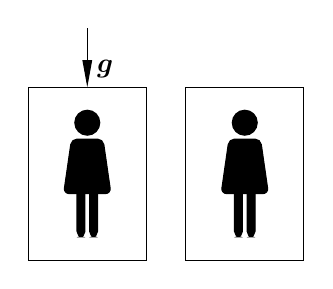
\begin{tikzpicture}
        \draw (-0.75cm,-1.75cm)--(0.75cm,-1.75cm)--(0.75cm,0.45cm)--(-0.75cm,0.45cm)--cycle;
        \node[circle,fill,minimum size=2.5mm] (head) {};
\draw[rounded corners=2pt,fill] ([shift={(-0.2cm,-1pt)}]head.south)--(-0.3cm,-0.9cm)--(0.3cm,-0.9cm)--([shift={(0.2cm,-1pt)}]head.south)--cycle;
\draw[rounded corners=2pt,fill] (-0.13cm,-0.6cm) rectangle (-0.03cm,-1.45cm);
\draw[rounded corners=2pt,fill] (0.13cm,-0.6cm) rectangle (0.03cm,-1.45cm);
\draw[->] (0,1.2cm) -- (0,0.45cm) node[above right]{$\vb*{g}$};
\begin{scope}[xshift=2cm]
\draw (-0.75cm,-1.75cm)--(0.75cm,-1.75cm)--(0.75cm,0.45cm)--(-0.75cm,0.45cm)--cycle;
        \node[circle,fill,minimum size=2.5mm] (head) {};
\draw[rounded corners=2pt,fill] ([shift={(-0.2cm,-1pt)}]head.south)--(-0.3cm,-0.9cm)--(0.3cm,-0.9cm)--([shift={(0.2cm,-1pt)}]head.south)--cycle;
\draw[rounded corners=2pt,fill] (-0.13cm,-0.6cm) rectangle (-0.03cm,-1.45cm);
\draw[rounded corners=2pt,fill] (0.13cm,-0.6cm) rectangle (0.03cm,-1.45cm);
\end{scope}
    \end{tikzpicture}
\end{document}